\documentclass[
   paper=a4,
   twoside=false,
   parskip=half,
   listof=entryprefix,
   listof=totoc,
   index=totoc,
   bibliography=totoc,
   headsepline,
]{scrbook}

\usepackage{silence}
\WarningFilter{biblatex}{File 'ngerman-iso.lbx'}
\WarningFilter{biblatex}{'\mainlang'}
\WarningFilter{biblatex}{Bibliography string 'online' untranslated}
\WarningFilter{hyperref}{Token not allowed in a PDF string}

%%%%%%%%%%%%%%%%%%%%%%%%%%%%%%%%%%%%%%%%%%%%%%%%%%%%%%%%%%%%%%%%%%%%%%%%%%%%%%
% Fonts Fonts Fonts
%%%%%%%%%%%%%%%%%%%%%%%%%%%%%%%%%%%%%%%%%%%%%%%%%%%%%%%%%%%%%%%%%%%%%%%%%%%%%%
\usepackage[utf8]{inputenc}
\usepackage[ngerman]{babel}
\usepackage[T1]{fontenc}

\usepackage{scrhack}
\usepackage{pdfpages,graphicx,subcaption,lastpage,xspace}
\graphicspath{ {./images} }
\usepackage{float,xcolor,csquotes,etoolbox}
\MakeOuterQuote{"}
\usepackage[automark,markcase=ignoreuppercase,autooneside=false]{scrlayer-scrpage}
\usepackage[official]{eurosym}
\usepackage[breaklinks,colorlinks,linkcolor=black,citecolor=black,filecolor=black,urlcolor=black]{hyperref}

%%%%%%%%%%%%%%%%%%%%%%%%%%%%%%%%%%%%%%%%%%%%%%%%%%%%%%%%%%%%%%%%%%%%%%%%%%%%%%
% Listings Paket
%%%%%%%%%%%%%%%%%%%%%%%%%%%%%%%%%%%%%%%%%%%%%%%%%%%%%%%%%%%%%%%%%%%%%%%%%%%%%%
\usepackage{listings,caption,pmboxdraw}
\definecolor{codebg}{rgb}{0.95,0.95,0.95}
\definecolor{lightgray}{rgb}{.9,.9,.9}
\definecolor{darkgray}{rgb}{.4,.4,.4}
\definecolor{purple}{rgb}{0.65, 0.12, 0.82}

\lstdefinelanguage{JavaScript}{
  keywords={break, case, catch, continue, debugger, default, delete, do, else, false, finally, for, function, if, in, instanceof, new, null, return, switch, this, throw, true, try, typeof, var, void, while, with, const},
  morecomment=[l]{//},
  morecomment=[s]{/*}{*/},
  morestring=[b]',
  morestring=[b]",
  ndkeywords={class, export, boolean, throw, implements, import, this},
  keywordstyle=\color{blue}\bfseries,
  ndkeywordstyle=\color{darkgray}\bfseries,
  identifierstyle=\color{black},
  commentstyle=\color{purple}\ttfamily,
  stringstyle=\color{red}\ttfamily,
  sensitive=true,
}
\lstset{
   basicstyle =\ttfamily\color{black}\small,
   keywordstyle =,
   commentstyle =\color{teal},
   stringstyle =\itshape,
   tabsize=2,
   breaklines=true,
   captionpos=b,
   breakatwhitespace,
   backgroundcolor={\color{codebg}},
   basewidth=0.5em,
   numbers=left,
   numberstyle=\tiny,
   numbersep=-8pt,
   language=JavaScript,
}

%%%%%%%%%%%%%%%%%%%%%%%%%%%%%%%%%%%%%%%%%%%%%%%%%%%%%%%%%%%%%%%%%%%%%%%%%%%%%%
% Bibliography
%%%%%%%%%%%%%%%%%%%%%%%%%%%%%%%%%%%%%%%%%%%%%%%%%%%%%%%%%%%%%%%%%%%%%%%%%%%%%%
\usepackage[
   backend=biber,
   urldate=long,
   style=iso-authoryear,
   useauthor=true,
   mincitenames=1,
   maxcitenames=3,
   maxbibnames=99,
]{biblatex}
\addbibresource{./bib/online.bib}
\addbibresource{./bib/book.bib}
\DeclareNameAlias{default}{family-given/given-family}

%%%%%%%%%%%%%%%%%%%%%%%%%%%%%%%%%%%%%%%%%%%%%%%%%%%%%%%%%%%%%%%%%%%%%%%%%%%%%%
% Fussnoten
%%%%%%%%%%%%%%%%%%%%%%%%%%%%%%%%%%%%%%%%%%%%%%%%%%%%%%%%%%%%%%%%%%%%%%%%%%%%%%
\deffootnote{1.5em}{1em}{\makebox[1.5em][l]{\thefootnotemark}}
\addtolength{\skip\footins}{\baselineskip}
\setlength{\dimen\footins}{10\baselineskip}
\interfootnotelinepenalty=10000  % Verhindert das Fortsetzen von Fussnoten

%%%%%%%%%%%%%%%%%%%%%%%%%%%%%%%%%%%%%%%%%%%%%%%%%%%%%%%%%%%%%%%%%%%%%%%%%%%%%%
% Commands
%%%%%%%%%%%%%%%%%%%%%%%%%%%%%%%%%%%%%%%%%%%%%%%%%%%%%%%%%%%%%%%%%%%%%%%%%%%%%%
\newcommand{\workDatum}{\today\xspace}
\newcommand{\workDateTime}{\today{} - \thistime\ Uhr}
\newcommand{\workFirma}{pep.digital GmbH\xspace}
\newcommand{\workTitel}{<Titel>}
\newcommand{\workNameStudent}{Marcel Maximilian Marek\xspace}
\newcommand{\workTyp}{Bachelorarbeit\xspace}

\newcommand{\www}[1]{\href{http://#1}{#1}}
\newcommand{\wwwhttp}[1]{\href{#1}{#1}}
\newcommand{\wwwlink}[1]{\footnote{\www{#1}}}

\newcommand{\zB}{\mbox{z.\,B.}\xspace}
\newcommand{\ua}{\mbox{u.\,a.}\xspace}
\newcommand{\dah}{\mbox{d.\,h.}\xspace}
\newcommand{\uAe}{\mbox{u.\,a.}\xspace}

\newcommand{\refp}[1]{Seite~\pageref{#1}\xspace}
\newcommand{\refk}[1]{Kapitel~\ref{#1}\xspace}
\newcommand{\refa}[1]{Abbildung~\ref{#1}\xspace}
\newcommand{\reft}[1]{Tabelle~\ref{#1}\xspace}
\newcommand{\reflst}[1]{Listing~\ref{#1}\xspace}

\newcommand{\engl}[1]{(engl: \textit{#1})\xspace}

%%%%%%%%%%%%%%%%%%%%%%%%%%%%%%%%%%%%%%%%%%%%%%%%%%%%%%%%%%%%%%%%%%%%%%%%%%%%%%
% Kopf und Fusszeilen
%%%%%%%%%%%%%%%%%%%%%%%%%%%%%%%%%%%%%%%%%%%%%%%%%%%%%%%%%%%%%%%%%%%%%%%%%%%%%%
\usepackage{scrtime}
\pagestyle{scrheadings}
\clearpairofpagestyles
\ihead[]{\leftmark \\ \rightmark} % Add \\ here to separate the left and right marks
\counterwithout{footnote}{chapter}
\ifoot[\workDateTime]{\workDateTime}
\ofoot[\pagemark]{\pagemark}


%%%%%%%%%%%%%%%%%%%%%%%%%%%%%%%%%%%%%%%%%%%%%%%%%%%%%%%%%%%%%%%%%%%%%%%%%%%%%%
% Acronyms
%%%%%%%%%%%%%%%%%%%%%%%%%%%%%%%%%%%%%%%%%%%%%%%%%%%%%%%%%%%%%%%%%%%%%%%%%%%%%%
% https://ctan.math.washington.edu/tex-archive/macros/latex/contrib/acro/acro-manual.pdf
\usepackage{acro,supertabular,array}

\acsetup{
   make-links=true,
   list/template=supertabular,
   list/heading=chapter*,
   list/sort=true,
   list/display=used,
   list/name=Abkürzungsverzeichnis,
}

\DeclareAcronym{html}{short=HTML,long=HyperText Markup Language}
\DeclareAcronym{js}{short=JS,long=JavaScript}

\usepackage{todonotes}

%%%%%%%%%%%%%%%%%%%%%%%%%%%%%%%%%%%%%%%%%%%%%%%%%%%%%%%%%%%%%%%%%%%%%%%%%%%%%%
% Glossar
%%%%%%%%%%%%%%%%%%%%%%%%%%%%%%%%%%%%%%%%%%%%%%%%%%%%%%%%%%%%%%%%%%%%%%%%%%%%%%
\usepackage[nonumberlist,toc]{glossaries}
\usepackage{glossary-super}
\setglossarystyle{super}
\makenoidxglossaries
\renewcommand*{\glstextformat}{\textbf}
\renewcommand*{\glsnamefont}{\textbf}
\setlength{\glsdescwidth}{0.8\linewidth}

\newglossaryentry{latex}
{
   name=Latex,
   description={Is a markup language specially suited
   for scientific documents}
}
\newglossaryentry{swagger}
{
   name=Swagger,
   description={Is a suite of tools for API developers from SmartBear Software and a former specification upon which the OpenAPI Specification is based}
}

%%%%%%%%%%%%%%%%%%%%%%%%%%%%%%%%%%%%%%%%%%%%%%%%%%%%%%%%%%%%%%%%%%%%%%%%%%%%%%
% Dokument
%%%%%%%%%%%%%%%%%%%%%%%%%%%%%%%%%%%%%%%%%%%%%%%%%%%%%%%%%%%%%%%%%%%%%%%%%%%%%%
\begin{document}

   \newcommand{\HRule}[2]{\noindent\rule[#1]{\linewidth}{#2}}
\newcommand{\vlinespace}[1]{\vspace*{#1\baselineskip}}
\newcommand{\titleemph}[1]{\textbf{#1}}
\begin{titlepage}
    \sffamily
    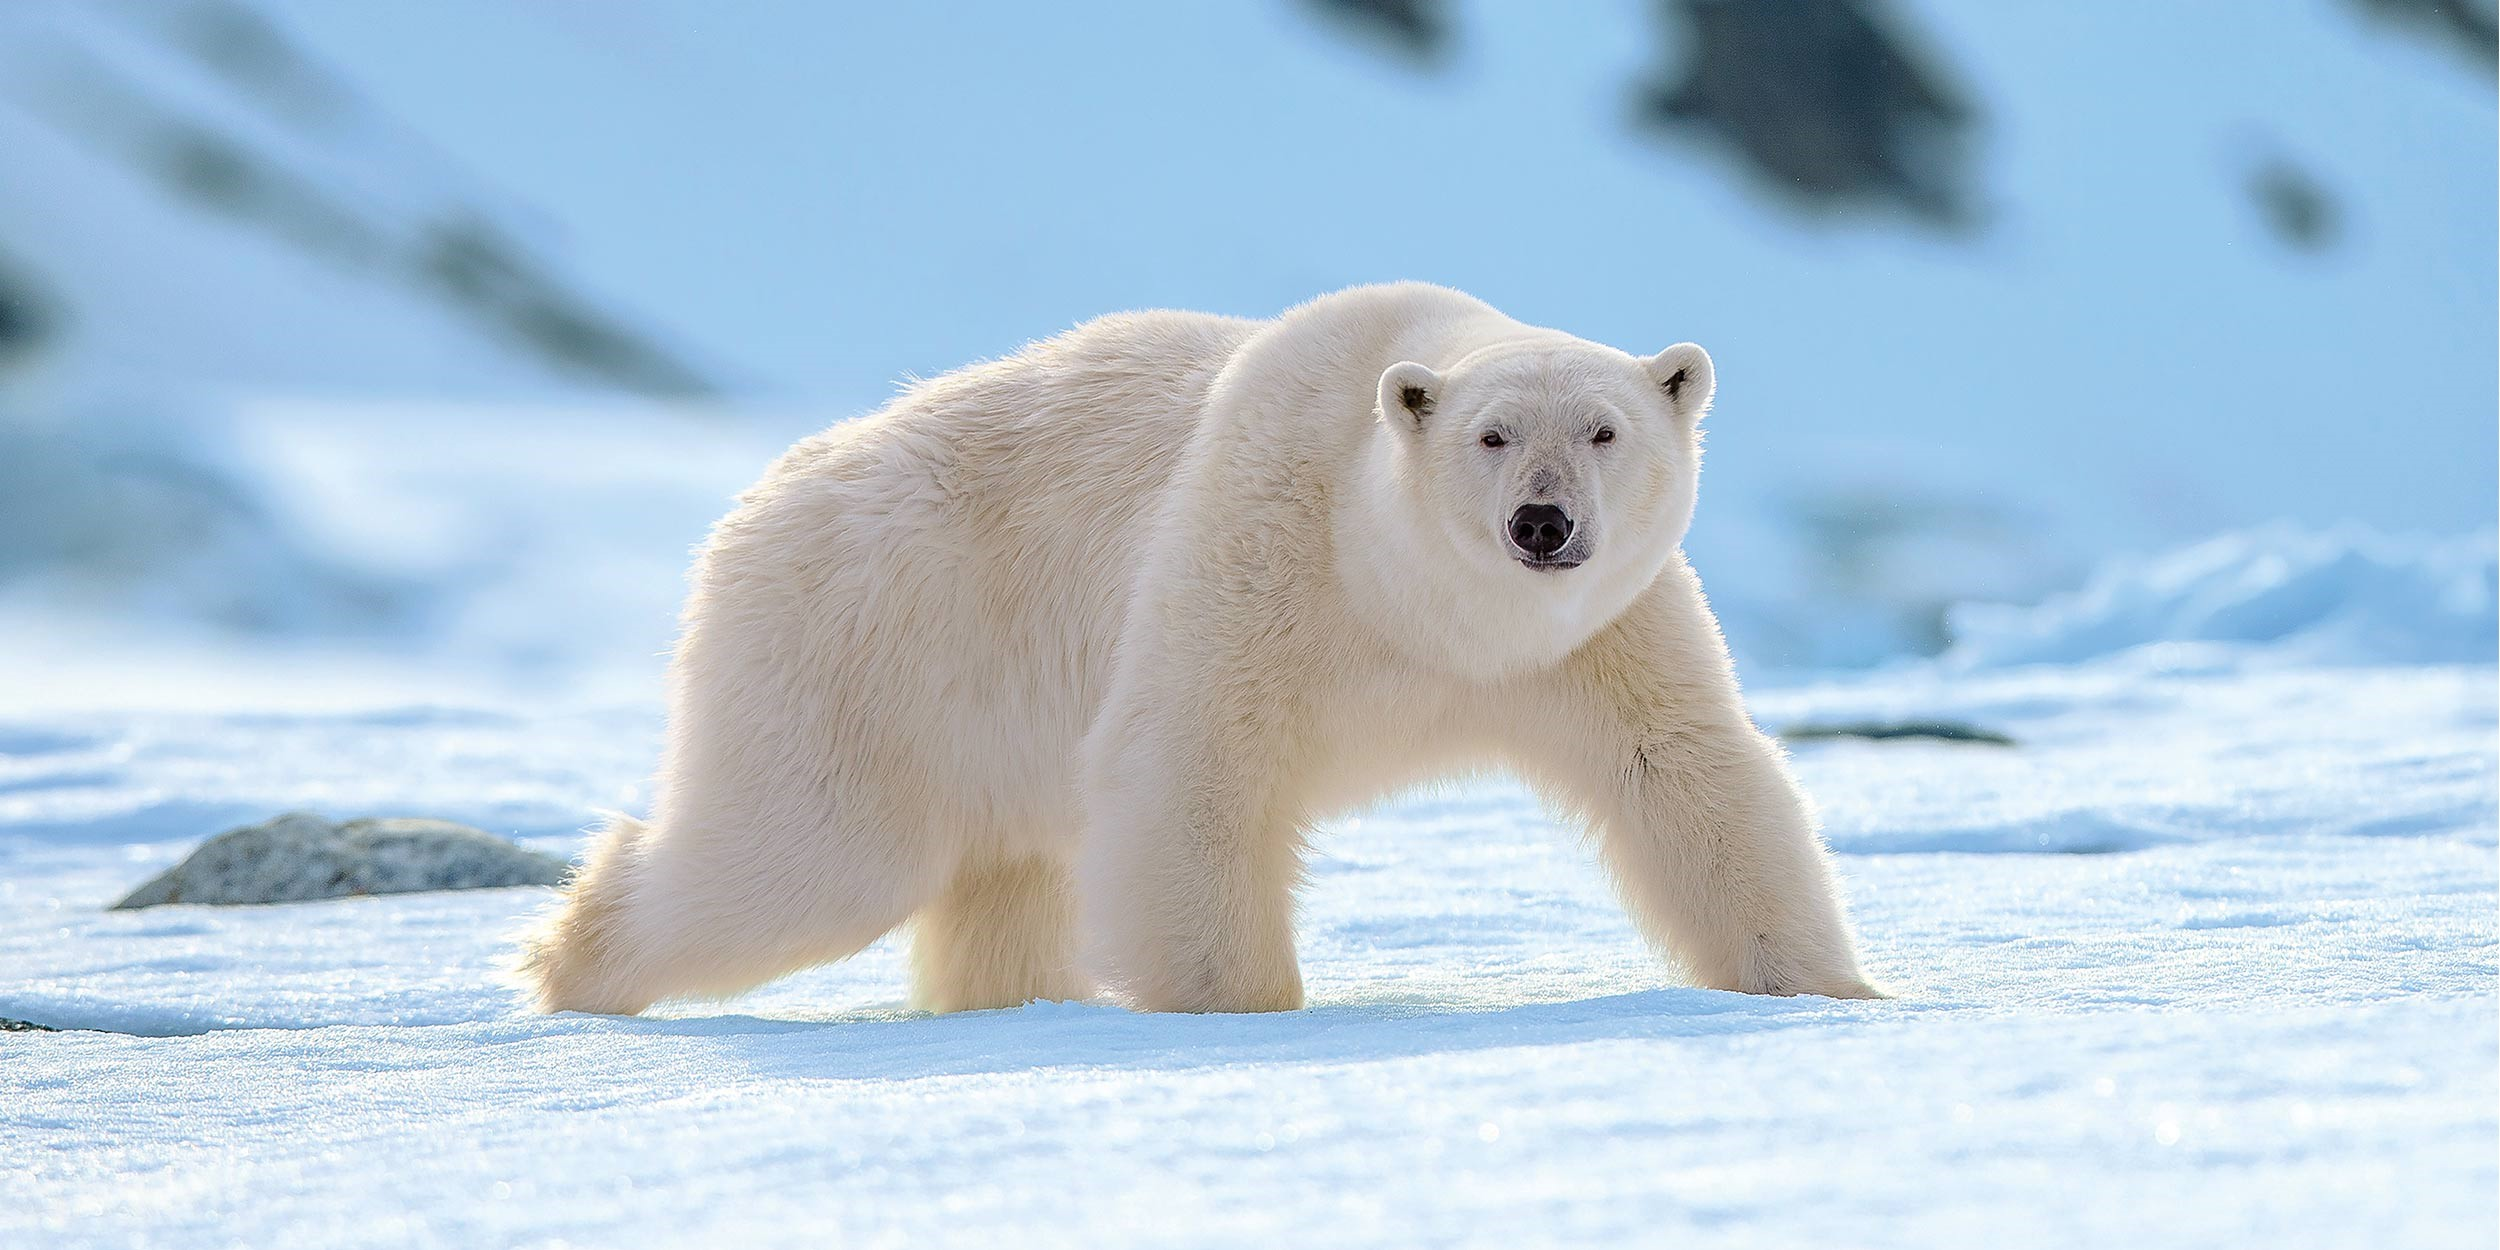
\includegraphics[width=5cm]{example}
    \hfill
    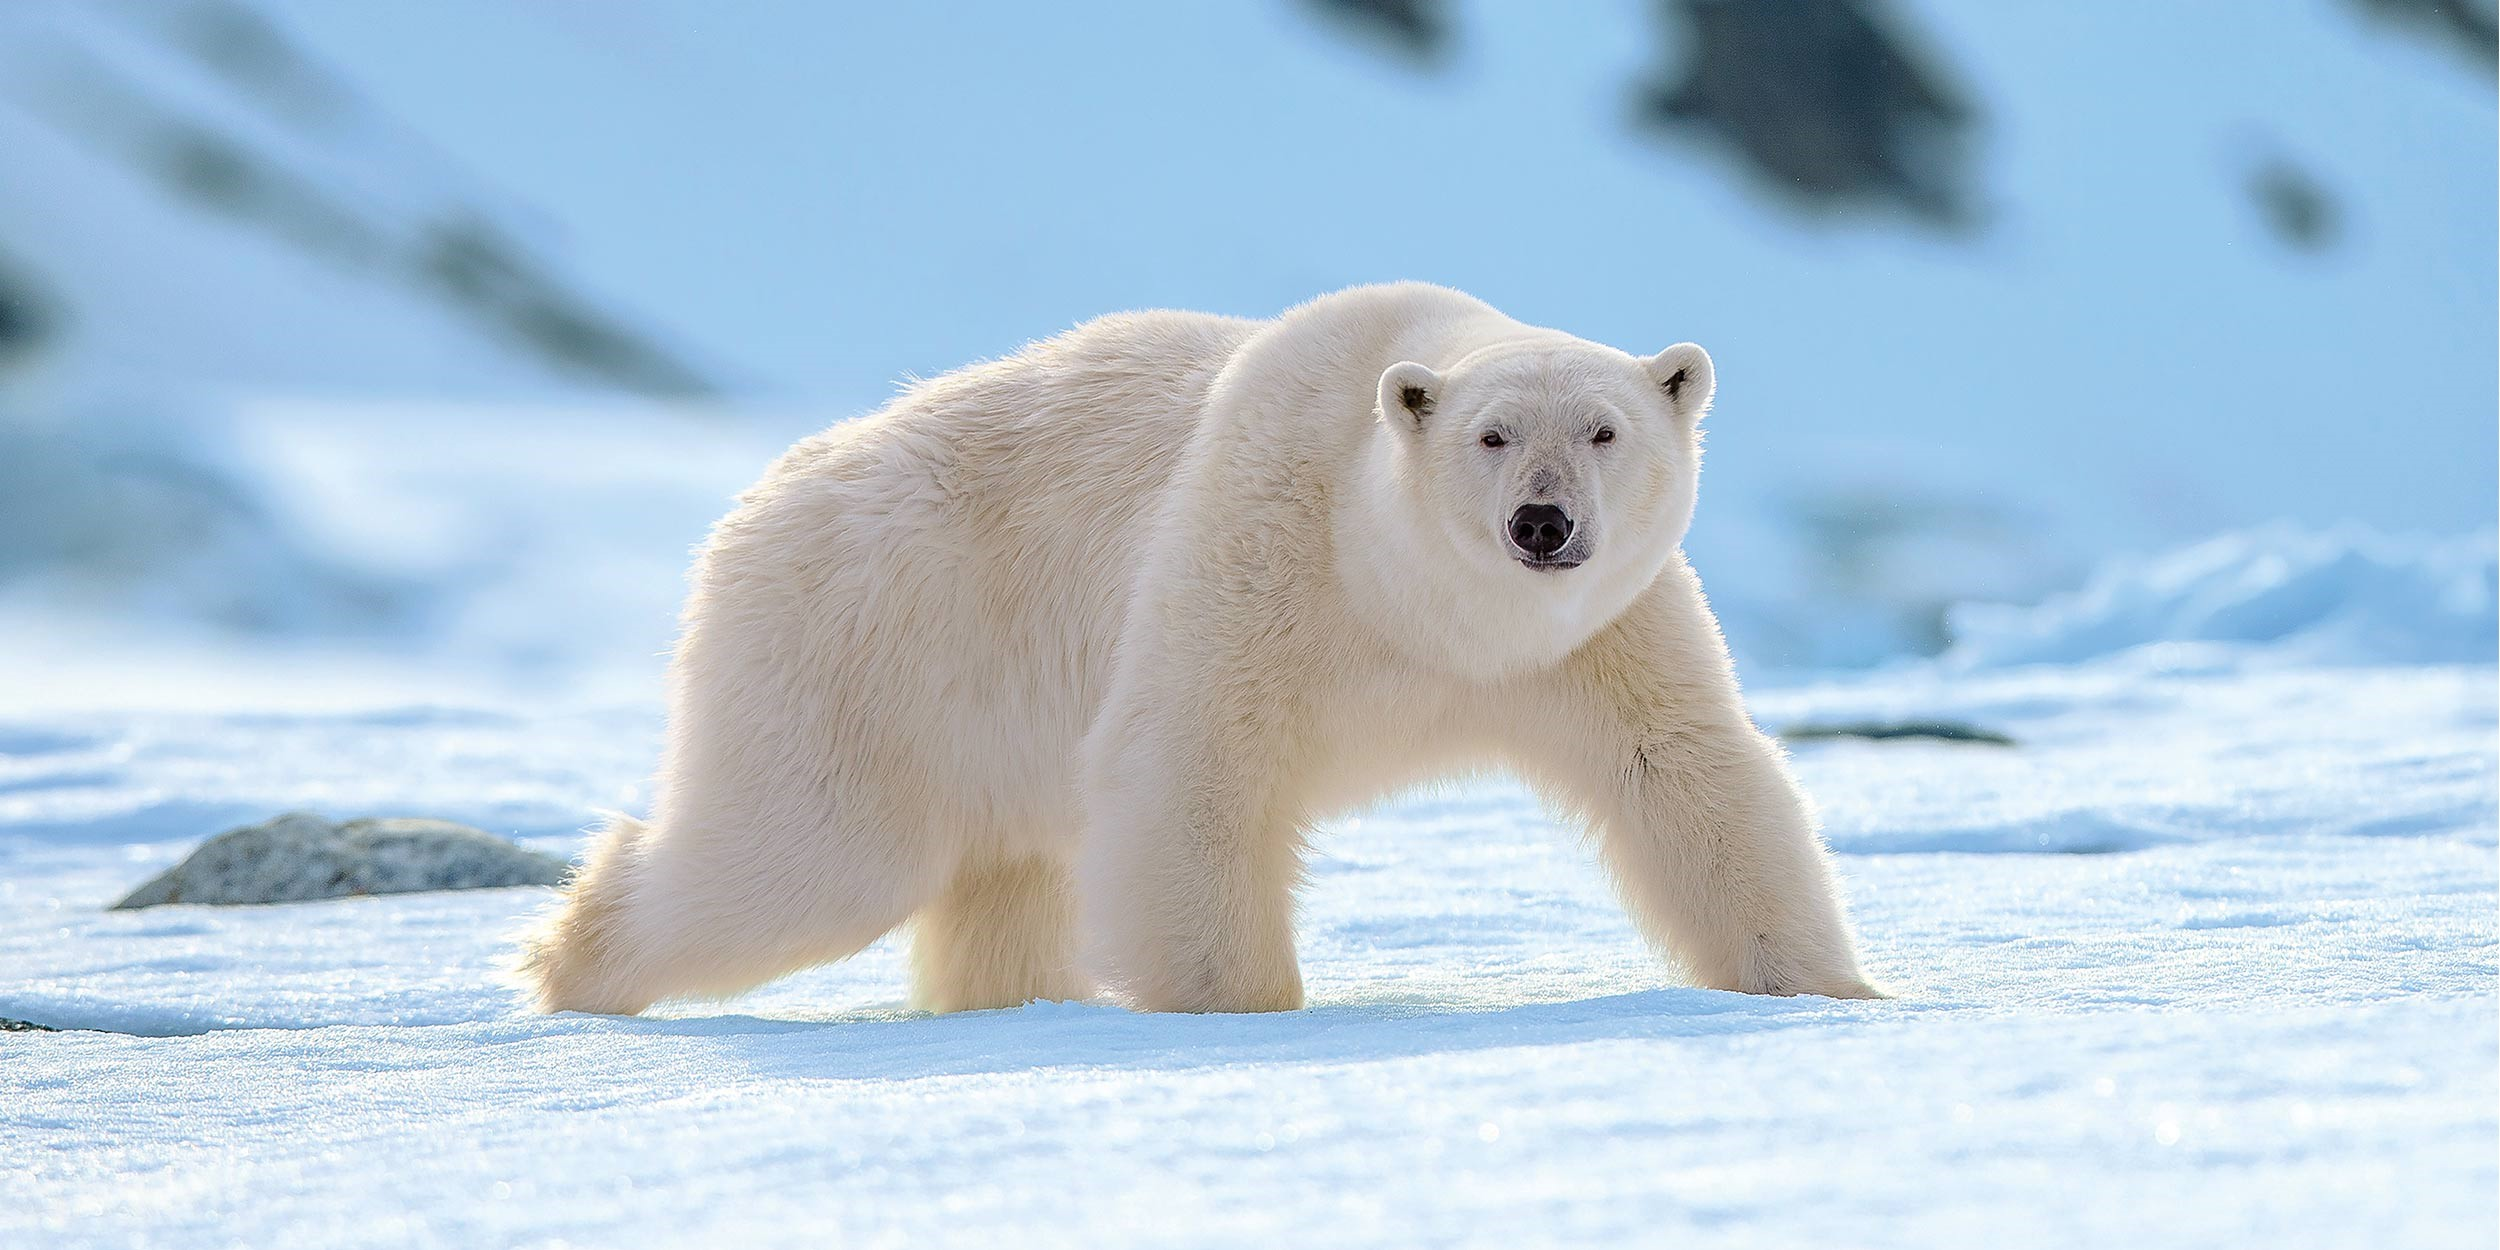
\includegraphics[width=5cm]{example}
    \HRule{13pt}{1pt}
    \centering
    \vlinespace{5}\\
    \workTyp\\
    \begin{Large}
        \textbf{Titel}\\
        \textbf{und mehr}\\
    \end{Large}
    \vlinespace{4}
    im Studiengang\\
    <Studiengang>\\
    am \workDatum\\
    \vlinespace{4}
    vorgelegt von\\
    \begin{Large}
        \textbf{\workNameStudent}\\
    \end{Large}
    \vlinespace{1}
    Matrikelnummer: <12345>
    \vfill
    \raggedright{}
    \HRule{13pt}{1pt} \\
    \titleemph{Erstprüfer:} Prof. <wx>\\
    \titleemph{Zweitprüfer:} Prof. <yz>
\end{titlepage}
   \chapter*{Eidesstattliche Erklärung}

Hiermit versichere ich, die vorliegende Arbeit selbstständig und unter ausschließlicher Verwendung der angegebenen Literatur und Hilfsmittel erstellt zu haben.

Die Arbeit wurde bisher in gleicher oder ähnlicher Form keiner anderen Prüfungsbehörde vorgelegt und auch nicht veröffentlicht.

\begin{tabbing}
          Esslingen, den \workDatum~~\= \rule{5cm}{0.3mm}\\
                                                                                                    \> Unterschrift
\end{tabbing}


   \tableofcontents
   \newpage
   \chapter{Einleitung}\label{chap:introduction}
\section{Hintergrund und Motivation}\label{sec:introduction-background-and-motiviation}

Im Rahmen der Arbeit wird eine webbasierte Labeling-Plattform zur Kennzeichnung von KI Daten als Prototyp realisiert. Die Plattform soll das schnelle Labeln von Bildern ermöglichen. Zum besseren Vergleich der Technologien, wird ein MEVN-Stack (Notiz für mich: oder nestjs statt express) verwendet. Dies bietet den Vorteil, dass der Softwarestack weit verbreitet ist und ein realistisches Anwendungsszenario geschaffen wird.
   \section{Zielsetzung der Arbeit}\label{sec:introduction-objectives}
Das Ziel ist es einen ''Computer Vision''-Datensatz zu erweitern, bis sich die Genauigkeit eines KI-Modells erhöht. Das Modell ist auf die Unterscheidung zwischen den beiden Gruppen ''Katze'' oder ''Hund'' trainiert.  Der Datensatzes teilt die Daten ebenfalls in ''Hund'' und ''Katze'' ein . Der Umgang mit Fehlern und Lücken soll untersucht werden und verschiedene Lösungsansätze zur Steigerung der Trefferquote angeboten werden. 

Dieses Projekt erarbeitet zur Überprüfung der erarbeiteten Lösungsansätzen eine Webplattform zur Bildkennzeichnung und -manipulation. Eine Mischung zwischen automatischen Lösungen und händischen Tools für die beschriftenden Mitarbeiter werden bereitgestellt. Inwiefern das KI-Modell nach der Bearbeitung durch die zur Verfügung gestellten Tools auf der Webseite höhere Trefferquoten erzielt, soll zweiter Untersuchungsgegenstand der Bachelorarbeit sein.

 Es resultieren drei Forschungsfragen, die zu untersuchen sind:

   Was sind die Ursachen für unvollständige Datensätze und welche Herausforderungen in Bezug auf Datenqualität und -integrität entstehen bei der Verarbeitung unvollständiger Datensätze?
   Ab welcher Anzahl von fehlenden Datenpunkten wird die Ergänzung mit zusätzlichen Daten empfohlen und was sind effektive Strategien zur Lösung von Datenlücken, wie etwa zusätzlicher Datenerfassung oder die Nutzung von externen Datenquellen? 
   Welche Werkzeuge sind verfügbar, um durch Datenbereinigung und -erweiterung die Trefferzahl zwischen 'Das ist ein Hund' oder 'Das ist eine Katze' zu erhöhen und wie kann die praktische Implementierung dieser Lösungsansätze erfolgen?
   Welche Auswirkungen haben Modifikationen eines Datensatzes auf die Lernrate und die Genauigkeit der Klassifizierung?
   ''Inwieweit kann Datenaugmentation die Qualität der Trainingsdaten verbessern?''


   \section{Aufbau der Arbeit}\label{sec:introduction-structure}
Die Arbeit stellt zuerst die unterschiedlichen Begrifflichkeiten des Themengebietes vor. Anschließend werden die Technologien vorgestellt und die dazugehörigen Evaluierungskriterien definiert. \\
Zuletzt wird in einer Fallstudie eine Webplattform gebaut und die Vor- und Nachteile/ Probleme und Lösungen beleuchtet.

   \newpage
   \include{sec:basics}
   \include{sec:basics-softwarestack-definition}
   \include{sec:basics-requirements}
   \include{sec:basics-overview-python}
   \include{sec:basics-overview-js}

   \newpage
   \chapter{Umgang mit unvollständigen Datensätzen}\label{sec:incomplete-data}
\section{Definition von vollständigen Datensätzen}
   \section{Ursachen für unvollständige Datensätze}\label{sec:incomplete-data-reason}

\subsection{Sensorausfälle oder -fehler}\label{sec:incomplete-data-sensor-errors}

\subsection{Fehlende Label}\label{sec:incomplete-data-missing-data}

\subsection{Datenverlust durch Übertragungsfehler}\label{sec:incomplete-data-data-loss}

\subsection{Menschliche Fehler in der Datenerfassung}\label{sec:incomplete-data-human-error}
   \section{Herausforderungen bei der Verarbeitung unvollständiger Datensätze}\label{sec:challenges}

\subsection{Datenqualität und -integrität}\label{sec:challenges-data-integrity}

\subsection{Auswirkungen auf maschinelles Lernen und KI-Modelle}\label{sec:challenges-impact-ai}

\subsection{Datenschutz- und Ethikaspekte}\label{sec:challenges-ethic}
   \section{Ansätze zur Erkennung von unvollständigen Datensätzen}\label{sec:recognition}

\subsection{Datenbereinigung}\label{sec:recognition-data-cleansing}

\subsection{Fehlererkennungsalgorithmen}\label{sec:recognition-error-detection-algorithms}

\subsection{Anomalieerkennungstechniken}\label{sec:recognition-anomaly}
   \section{Strategien zur Lösung von Datenlücken}\label{sec:data-gaps}

\subsection{Datenerfassung und -annotation}\label{sec:data-gaps-acquisition}

\subsection{Interpolation und Extrapolation}\label{sec:data-gaps-interpolation}

\subsection{Nutzung von externen Datenquellen}\label{sec:data-gaps-external-sources}
   \section{Praktische Implementierung von Lösungsansätzen}\label{sec:solution}

\subsection{Fallstudien und Beispiele}\label{sec:solution-examples}

\subsection{Auswahl geeigneter Werkzeuge und Bibliotheken}\label{sec:tools}


   \section{Evaluierung der Effektivität von Lösungsansätzen}\label{sec:evaluierung}

\subsection{Metriken zur Bewertung der Datenqualität}\label{sec:evaluierung-metrix}

\subsection{Vergleich unterschiedlicher Strategien}\label{sec:evaluierung-comparsion}

\subsection{Fallbeispiele aus der Industrie}\label{sec:evaluierung-examples}



   \newpage
   \chapter{Analyse und Vergleich relevanter Softwarestacks}\label{sec:stack-a}
\section{Softwarestack A: Vor- und Nachteile}
   \chapter{Design and Implementation}
-> Datensätze vorstellen
-> Tensorflow Project überprüfen

math.confusion:matrix .> erkennen falscher bilder

neue  Gliederung -> Mit Koch absprechen / Neuer Termin mit Koch
-> Neuer Termin mit Koch 
-> Schauen, dass das Thema noch nicht "erforscht" wurde
-> Hat es Vorteile Daten zu verbessern?
-> Wie verhalten sich Daten, wenn man spiegelt / manipuliert
-> Wie verbessert sich die learning rate?
-> Die große herausforderung sind sinnvolle Trainingsdaten zu bekommen - Wir bauen ein Toll und schauen was rauskommt.
-> Forschungsfragen auf zwei reduzieren
1. Tool Plattform 2. Funktionen Augmentation (Spiegeln, automatisch Suchen)Beschreiben was wir gedacht haben, wieso zum Vervollständigen gewählt. Welches dieser Verfahren ist das beste. Wie bekomme ich saubere Datenlage? 

Forschungsfragen können allgemeiner sein
-> Welche Ansätze gibt es
-> Nicht fest Datensatz festlegen (Klassenunterscheidung statt "Hund" und "Katze") -> Wieviel Prozent sind notwendig, um zu unterscheiden zu können
-> Mehr Fokus auf Augmentation statt Labeling Plattform
-> Alle kritischen Stellen rauswerfen

Forschungsfrage: Vergleich unterschiedlicher MEthoden zur Augmentation
Forschungsfrage: Erst bei Interpretation statistischer Teil. Ergebnis neutral.  

tensorflow gute bücher
Gibt es eventuell schon viel zu viele papers -> nicht genau meins, sondern andere richtung. Ist das gut oder schlecht?

Data Scraping gibt es schon eine BA? -> Warum BA

Zielsetzung der Arbeit gut? Vorlesen

Zuviele Forschungsfragen? -> Soll nur "Was gibt es als Lösungsansätze" als Forschungsfrage, wollte professioneller klingen.

Hintegrund und Motivation -> Durch den Anwendungsfall innerhalb der Firma pep.digital werden die Mitarbeiter beim Labeln helfen (daher Webplattform gewählt)

-> ggbfs als Quelle auch BA -> Quelle in BA nachschauen

-> Zügig klarheit geschaffen und koch befragen (scope hat sich geändert)


   \newpage
   \chapter{Fallstudie: Entwicklung einer Labeling Plattform}\label{sec:anforderungsanalyse}
\section{Anforderungsanalyse für die zu entwickelnde Plattform}

Wie weit / abgeschlossen ist die Technologie

Bilder müssen in der gleichen Größe hinterlegt werden. Eine Funktion die Bilder auf den selbigen Bildbereich zuschneiden oder vergrößern zu können, ist unabdingbar.

Daten mit Verzerrungen oder Rauschen müssen extra auf überwacht werden. Es ist sinnvoll eine Möglichkeit zur Verfügung zu stellen, bei der Trainingsdaten mit beschriebenen Merkmalen gekennzeichnet werden können. Eine Fourier-Transformation / Gaußsche Glättung des Signals kann das Rauschen verringern.

Falls möglich, sollten die Freiheitsgrade verringert werden, um unnötige Datenmengen zu verringern. Die Verringerung der Freiheitsgrade muss auf die einzelnen Fälle abgestimmt werden, da ähnliche Elemente nicht mehr erkannt werden können sollte zu sehr generalisiert werden. Ein Beispiel einer zu hohen Verringerung wären einzelne Klassen bei der Buchstabenerkennung (bei n und h).

Für einen möglichst einfachen und natürlichen Weg einen Treffer zu messen, kann die Hamming Distanz verwendet werden (\cite[][]{cv-principles-link}). Eine geringe Hamming Distanz bedeutet, dass eine hohe Übereinstimmung besteht.

Desweiteren können Bilder auch in gedrehter Form gespeichert sein. Dies sorgt für keine Übereinstimmung obwohl die Bilder identisch wären. Zur Vorbeugung können Referentlinien (T beispielsweise eine horizontale und eine vertikale Linie) verwendet werden und die Bilder vorab in die richtige Position gedreht werden.

Außerdem können die Bilder außerhalb des Bildzentrums liegen. Dies erhöht die Freiheitsgrade unnötig. Eine Funktion zum Zentrieren des Bildes ist wünschenswert. 

Einordnen in Gruppierung als Datenpunkt.


Kontrasterhöhung um Bildbereiche/ Elemente besser erkennen zu können.
-> Graustufen Gewichtung:
HDTV Formula ("0.21×Red + 0.72×Green + 0.07×Blue")
PAL/NTSC Formula( "0.30×Red + 0.59×Green + 0.11×Blue")

Link: \url{https://web.s.ebscohost.com/ehost/ebookviewer/ebook/bmxlYmtfXzEyMDQyODlfX0FO0?sid=7eaf4273-b0ca-4e23-af7e-c46da0867380@redis&vid=0&lpid=lp_iii&format=EB}


   \section{Architektur und Design der Plattform}\label{sec:architektur}
   \section{Implementierung und Umsetzung}\label{sec:implementierung}
   \label{sec:testing}
\section{Testing und Validierung}
   \label{sec:herausforderungen}
\section{Erfahrungen und Herausforderungen während der Entwicklung}

   \newpage
   \chapter{Bewertung und Schlussfolgerungen}\label{sec:bewertung}
\section{Bewertung der ausgewählten Softwarestacks anhand der Evaluierungskriterien}
   \label{sec:bewertung-vergleich-anforderungen}
\section{Vergleich der entwickelten Plattform mit den Anforderungen}
   \section{Erkenntnisse und Empfehlungen für die Auswahl zukünftiger Softwarestacks}\label{sec:erkenntnisse}
   \label{sec:fazit}
\section{Fazit und Ausblick}

   \listoffigures
   \renewcommand\lstlistingname{Codefragment}
   \renewcommand\lstlistlistingname{Codeverzeichnis}
   \lstlistoflistings
   \printacronyms[heading=addchap]
   \printnoidxglossary
   \section{Example}

\begin{figure}[H]
    \begin{center} 
        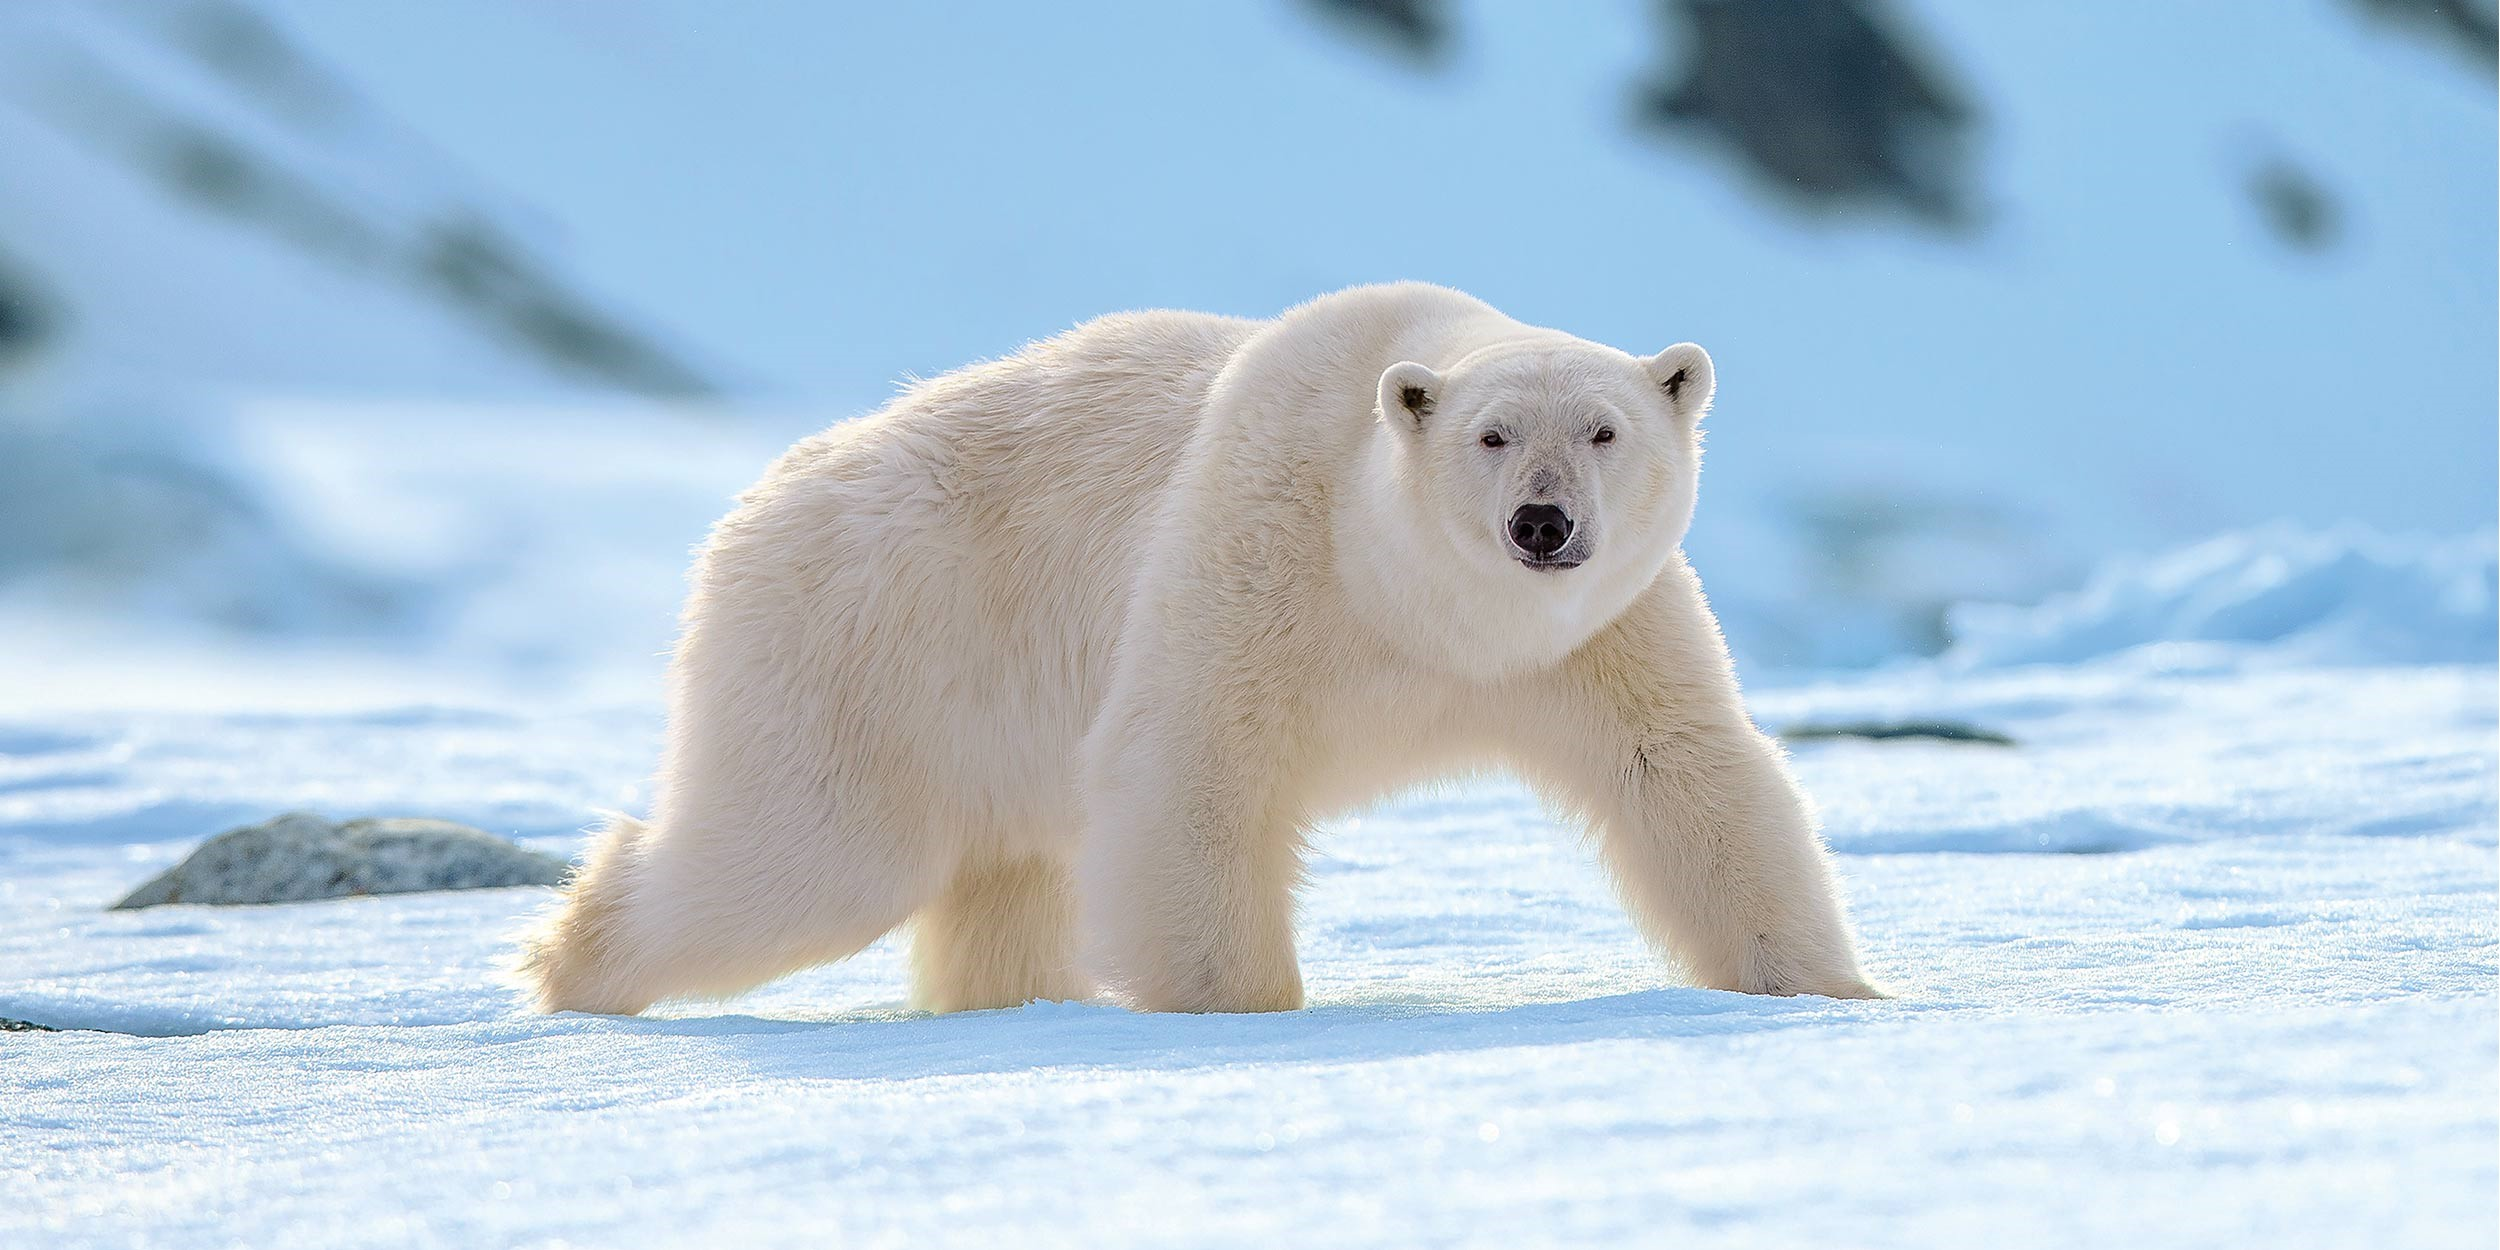
\includegraphics[width=0.8\textwidth]{example}
        \caption{Example Image}
        \label{fig:example}
    \end{center}
\end{figure}

\cite[vgl. dazu][]{example-book}

\cite[vgl. dazu][]{example-online}

\newpage

\begin{lstlisting}[language=Bash]
#!/bin/bash

echo "Hello World"
\end{lstlisting}

\begin{lstlisting}[language=Python]
# same in python

print("Hello World")
\end{lstlisting}

\begin{verbatim}
$ sudo apt-get update
$ sudo apt-get install python
\end{verbatim}


   \printbibheading[title=Literaturverzeichnis]
   \printbibliography[type=book,heading=subbibliography,title=Buch-Quellen]
   \printbibliography[type=online,heading=subbibliography,title=Online-Quellen]


   
\end{document}
